\documentclass[12pt,letterpaper]{article}
\usepackage[top=0.85in,left=2.75in,footskip=0.75in,marginparwidth=2in]{geometry}

% use Unicode characters - try changing the option if you run into troubles with special characters (e.g. umlauts)
\usepackage[utf8]{inputenc}
\usepackage{array,amsmath}

% clean citations
\usepackage{cite}
\usepackage{float}

% hyperref makes references clicky. use \url{www.example.com} or \href{www.example.com}{description} to add a clicky url
\usepackage{nameref,hyperref}

% line numbers
\usepackage[right]{lineno}

% improves typesetting in LaTeX
\usepackage{microtype}
\DisableLigatures[f]{encoding = *, family = * }

% text layout - change as needed
\raggedright
\setlength{\parindent}{0.5cm}
\textwidth 5.25in 
\textheight 8.75in

% Remove % for double line spacing
%\usepackage{setspace}  
%\doublespacing

% use adjustwidth environment to exceed text width (see examples in text)
\usepackage{changepage}

% adjust caption style
\usepackage[aboveskip=1pt,labelfont=bf,labelsep=period,singlelinecheck=off]{caption}

% remove brackets from references
\makeatletter
\renewcommand{\@biblabel}[1]{\quad#1.}
\makeatother

% headrule, footrule and page numbers
\usepackage{lastpage,fancyhdr,graphicx}
\usepackage{epstopdf}
\pagestyle{myheadings}
\pagestyle{fancy}
\fancyhf{}
\rfoot{\thepage/\pageref{LastPage}}
\renewcommand{\footrule}{\hrule height 2pt \vspace{2mm}}
\fancyheadoffset[L]{2.25in}
\fancyfootoffset[L]{2.25in}

% use \textcolor{color}{text} for colored text (e.g. highlight to-do areas)
\usepackage{color}

% define custom colors (this one is for figure captions)
\definecolor{Gray}{gray}{.25}

% this is required to include graphics
\usepackage{graphicx}

% use if you want to put caption to the side of the figure - see example in text
\usepackage{sidecap}

% use for have text wrap around figures
\usepackage{wrapfig}
\usepackage[pscoord]{eso-pic}
\usepackage[fulladjust]{marginnote}
\reversemarginpar

% document begins here
\begin{document}
\vspace*{0.35in}

% title goes here:
{\Large
\textbf{\newline Estimating the Optimal Lysogenic Propensity in Stressed Environments}
}
\newline
% authors go here:
\\
\noindent {\large Devang Thakkar, and Supreet Saini}
\vspace{1mm}
\\
\noindent Indian Institute of Technology Bombay, Mumbai 400076, India
\\

\section*{Abstract}
\par Having infected a bacterial cell, a temperate phage has to make a choice between (a) integrating itself into the bacterial genome, i.e. \textit{lysogeny}, and (b) using the bacterial machinery to create multiple copies of itself and lysing the cell in the process, i.e. \textit{lysis}. In order to maximize its long-term growth rate, phages need to ensure that they do not wipe off their bacterial hosts. Temperate phages have been observed to exhibit lysogenic propensities dependent on the MoI (Multiplicity of Infection), among other factors. We propose a model to estimate the propensity of lysogeny opted for by the phages in order to maximize coexistence. One possible approach to do so is to adopt a strategy that would help to attain and maintain an approximately equal proportion of phages with respect to their host. We find that the optimal fraction of phages opting for lysogeny follows a sigmoidal relationship with the MoI and is comparable to results obtained experimentally. We further assess the impact of phage and bacterial environmental stresses on the lysogenic propensity. Our results indicate that the optimal value of lysogenic propensity is greatly dependent on the  intensity of these stresses.

% now start line numbers
\linenumbers

\section*{Introduction}
The primary aim of an organism is to avoid extinction, and to this end, it produces as many progenies as it is able to. Ideally, bacteriophages must then opt only for lysis constantly without ever opting for lysogeny - an alternative that is less beneficial that than the former. This indeed is the best strategy in the span of a few epochs, however, survival in the long run is dependent on the coexistence of their prey - the bacteria \cite{de2006viruses}, \cite{weitz2005coevolutionary}, \cite{echols1972developmental}. Temperate phages \cite{stewart1984population}, \cite{maslov2015well} are thus phages that strike a balance between lysis and lysogeny in order to maximize long term survival. We consider below a simplistic model that explains how a temperate phage maximizes its survival in the long run.

\newpage

\section*{Materials and Methods}

Besides being characterized by the relative populations and growth rates, the phage bacteria ecosystem implemented in our model is also dependent on the environmental stresses. We model the environmental stresses as the probability of 'good' and 'bad' environments for each of the species. Good environments favors the growth of the species while bad environments triggers an exponential decay of the species. A good environment for the free phages is one wherein the phage population may undergo lysis and increment the number of free phages. On the other hand, a bad free phage environment involves an exponential decay of the free phage population. Correspondingly, a good bacterial environment allows normal replicative growth of the bacterial population whereas a bad bacterial environment leads to an exponential decay of uninfected and lysogenized bacteria alike. The probability of a good environment for the phage and bacterial population is denoted by $p_1$ and $p_2$ respectively.

\subsection*{Assumptions}
The relative population strength of the phages with respect to the bacteria is indicated by the MoI. The notion of MoI antedates the theory of phage infection commonly accepted today - that the adsorption of phages onto the bacteria follows a Poisson distribution \cite{ellis1939growth}. Historically, MoI had been defined as the ratio of number of phages to the number of bacteria \cite{kasman2002overcoming},\cite{abedon2016phage}. However, over the years, scientists have coined various terminologies such as $MoI_{actual}$, $MoI_{input}$, and $API$ \textit{(Average Phage Input)} to represent this quantity more precisely. For our discussion, we consider MoI to be the ratio of the effective number of phages (free phages + lysogenized phages) to the number of bacteria in the system.

\begin{equation}
\label{eq1}
MoI = \frac{Free\;phages + Lysogenized\;phages}{Healthy\;bacteria + Infected\;bacteria}
\end{equation}

Secondly, we consider the infection of the bacteria by the phages to be quantified by a Poisson distribution with a mean equal to the MoI. This implies that for $N$ bacteria that are exposed to phages at an MoI of $m$, $N*e^{-m}$ bacteria are not infected and would still be counted as healthy bacteria. Thirdly, we assume that for multiple infections of a bacterial cell, only one of the phages is effectively active\cite{ellis1939growth}. A corollary of this is that the number of lysogenized phages can be considered to be equal to the number of infected bacteria. Following from Eq. \ref{eq1}, we thus get

\begin{equation}
\label{eq2}
MoI = \frac{Free\;phages + Infected\;bacteria}{Healthy\;bacteria + Infected\;bacteria}
\end{equation}

\subsection*{Notation}
Table \ref{tab1} lists the notation and the values of the parameters of our model.

\begin{table}[!ht]
\setlength\extrarowheight{5pt}
% \begin{adjustwidth}{-1.5in}{0in} % comment out/remove adjustwidth environment if table fits in text column.
\centering
\caption{{\bf List of parameters:} This table lists out all the parameters in the model along with their symbol and values.}
\begin{tabular}{|l|l|r|}
\hline
\multicolumn{1}{|l|}{\bf Symbol} & \multicolumn{1}{|l|}{\bf Parameter} & \multicolumn{1}{|r|}{\bf Value(s)}\\[5pt] \hline
$MoI$ & Multiplicity of Infection & [0.01, 0.02, ..., 2] \\[5pt] \hline
$N_{b,h}$ & Number of uninfected bacteria & 10000 (Initial) \\[5pt] \hline
$N_{b,i}$ & Number of infected bacteria & 0 (Initial) \\[5pt] \hline
$N_{p,f}$ & Number of free phages & $N_{b,h}*MoI$ \\[5pt] \hline
$\gamma$ & Replicative growth rate & \{1*, 2, 5\} \\[5pt] \hline
$\alpha$ & Lytic burst rate & \{10*, 20\} \\[5pt] \hline
$p_1$ & Probability of good phage environment & [0.1, 0.2, ..., 1.0] \\[5pt] \hline
$p_2$ & Probability of good bacterial environment & [0.1, 0.2, ..., 1.0] \\[5pt] \hline
$\lambda_{p}$ & Phage decay rate in bad environments & \{1, 2, 3\} \\[5pt] \hline
$\lambda_{b}$ & Bacterial decay rate in bad environments & \{0.1, 1\} \\[5pt] \hline
$P_{lyso}$ & Lysogenic propensity & To be calculated \\[5pt] \hline
\end{tabular}
\label{tab1}
% \end{adjustwidth}
\end{table}
(* - Chosen)

\subsection*{The Model}
Traditionally, stochastic simulations using the Gillespie Algorithm \cite{gillespie1977exact} have been carried out in order to understand the working of the lysis-lysogeny decision \cite{cao2010probability}, \cite{trinh2017cell}. Using this method requires us to consider a population with infinitely many bacteria since the phages grow exponentially faster compared to the bacteria. \\

Our model circumvents this problem by considering a single epoch simulation of the phage-bacteria interaction. We hypothesize that one way in which the phages may ensure their long-term survival is by striving for an approximately equal phage to bacterium ratio. In other words, the optimal strategy would be to choose the magnitude of the lysogenic propensity to be such that the resulting MoI is closest to unity. The interaction is modeled using the set of equations Eq. \ref{eq3} to Eq. \ref{eq14} :

\newpage

\subsubsection*{Good $p_1$, Good $p_2$}
\begin{gather}
\frac{dN_{b,h}}{dt} = \gamma\,N_{b,h} - N_{p,f}\,(1-e^{-MoI}) \label{eq3} \\
\frac{dN_{b,i}}{dt} = \gamma\,N_{b,i} + P_{lyso}\,N_{p,f}\,(1-e^{-MoI}) \label{eq4} \\
\frac{dN_{p,f}}{dt} = \alpha\,(1-P_{lyso})\,N_{p,f}\,(1-e^{-MoI}) - P_{lyso}\,N_{p,f} \label{eq5}
\end{gather}

\subsubsection*{Good $p_1$, Bad $p_2$}
\begin{gather}
\frac{dN_{b,h}}{dt} = \gamma\,N_{b,h} - N_{p,f}\,(1-e^{-MoI}) \label{eq6} \\
\frac{dN_{b,i}}{dt} = [\gamma\,N_{b,i} + P_{lyso}\,N_{p,f}\,(1-e^{-MoI})]\,e^{-\lambda_b} \label{eq7} \\
\frac{dN_{p,f}}{dt} = \alpha\,(1-P_{lyso})\,N_{p,f}\,(1-e^{-MoI}) - P_{lyso}\,N_{p,f} \label{8}
\end{gather}

\subsubsection*{Bad $p_1$, Good $p_2$}
\begin{gather}
\frac{dN_{b,h}}{dt} = \gamma\,N_{b,h} - N_{p,f}\,(1-e^{-MoI}) \label{eq9} \\
\frac{dN_{b,i}}{dt} = \gamma\,N_{b,i} + P_{lyso}\,N_{p,f}\,(1-e^{-MoI}) \label{eq10} \\
\frac{dN_{p,f}}{dt} = [\alpha\,(1-P_{lyso})\,N_{p,f}\,(1-e^{-MoI}) - P_{lyso}\,N_{p,f}]\,e^{-\lambda_p} \label{eq11}
\end{gather}

\subsubsection*{Bad $p_1$, Bad $p_2$}
\begin{gather}
\frac{dN_{b,h}}{dt} = \gamma\,N_{b,h} - N_{p,f}\,(1-e^{-MoI}) \label{eq12} \\
\frac{dN_{b,i}}{dt} = [\gamma\,N_{b,i} + P_{lyso}\,N_{p,f}\,(1-e^{-MoI})]\,e^{-\lambda_b} \label{eq13} \\
\frac{dN_{p,f}}{dt} = [\alpha\,(1-P_{lyso})\,N_{p,f}\,(1-e^{-MoI}) - P_{lyso}\,N_{p,f}]\,e^{-\lambda_p} \label{eq14}
\end{gather}

\subsection*{Simulation}
Our aim here is to use the aforementioned equations and identify the optimal curve in the $P_{lyso}$ - $MoI$ space for each value of the tuple $(p_1,p_2)$ in the appropriate range. 
\begin{enumerate}
\item For each value of the probabilities $p_1$ and $p_2$ indicated in Table \ref{tab1}, we establish a random phage and bacterial environment.
\item Next, we calculate the resulting MoI based on a single epoch resolution of the set of equations \ref{eq3}-\ref{eq14}.
\item The value of $P_{lyso}$ that results in an MoI closest to unity is chosen. 
\end{enumerate}
Steps 1-3 are repeated multiple times and the average value of the optimal $P_{lyso}$ is calculated. (Note: Initially, the number of iterations was set to 1000, however it was later increased to 3000 in order to obtain a smoother estimate of $P_{lyso}$ in bad environments.) The scripts for this simulation are available at (add link to Github after updating completely)

\section*{Results}
\textbf{The trend of the optimal lysogenic propensity}\newline

The plot in Figure \ref{fig1} shows the mean trend and maximum deviations of the optimal propensity of lysogeny for two extreme values of $p_1$ as a function of $MoI$ for variations in $p_2$ (the probability of a good bacterial environment), $\lambda_b$ (the bacterial decay rate), $\lambda_p$ (the phage decay rate). The plot illustrates the robustness of the estimated $P_{lyso}$ for variation in the aforementioned parameters over the ranges mentioned in Table \ref{tab1}. % avoid blank space here 
\marginpar{
\vspace{1.0cm} % adjust vertical position relative to text with \vspace{} - note that you can enter negative numbers to move margin caption up
\color{Gray} % this gives caption a grey color to set it apart from text body
\textbf{Figure \ref{fig1}. $P_{lyso}$ as a function of $MoI$:} % note that \ref{fig1} refers to the corresponding wrapfigure
The blue curve refers to the mean values when $p_1$ = 0.2, whereas the red curve refers to the mean values when $p_1$ = 0.8; the shaded area represents the variation due to changes in $p_2$, $\lambda_p$, and $\lambda_b$.}

\begin{wrapfigure}[15]{l}{75mm}
% the number in [] of wrapfigure is optional and gives the number of text lines that should be wrapped around the text. Adjust according to your figures height
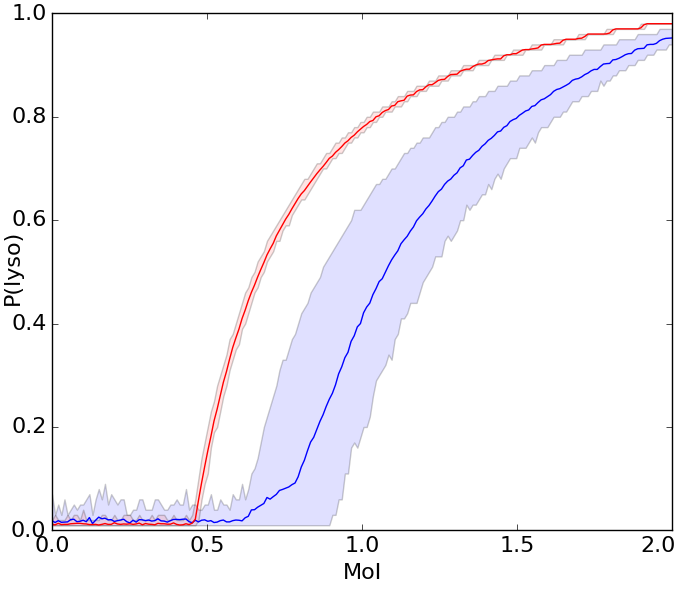
\includegraphics[width=75mm]{combo.png}
\captionsetup{labelformat=empty} % makes sure dummy caption is blank
\caption{} % add dummy caption - otherwise \label won't work and figure numbering will not count up
\label{fig1} % use \ref{fig1} to reference to this figure
\end{wrapfigure}% avoid blank space here
As seen from Figure \ref{fig1}, the optimal strategy is to opt entirely for lysis as long as the relative phage concentration in the environment is low. 

For a bad phage environment, represented by the blue curve, the relation is affected more by changes in other parameters than a good phage environment - shown by the red curve with an extremely thin error area. Classically, the environment has been assumed to be good, thus missing out on the variation caused by changes in the values of the parameters in bad environments. It is interesting to note that as the environment becomes worse for phages, the lysogenic propensity at a given $MoI$ decreases. This follows from the fact that, for an environment where the phages are rapidly dying, the phages need to produce a higher number of progeny in order to avoid being wiped off in the long run. Oddly enough, the change in the bacterial environment does not seem to affect the trend of lysogenic propensity as greatly as the change in the phage environment.

This may be attributed to the fact that the population of uninfected bacteria is much more than that of lysogenized bacteria that are affected by bad bacterial environments. Consequently, the effects of bad bacterial environments are not as severe as that of bad phage environments. These observations are evident from Figure \ref{fig2} which illustrates the relation between $P_{lyso}$ and $MoI$ for a matrix of values of probabilities $p_1$ and $p_2$.

\begin{figure}[H]
\hspace*{-1.05in}
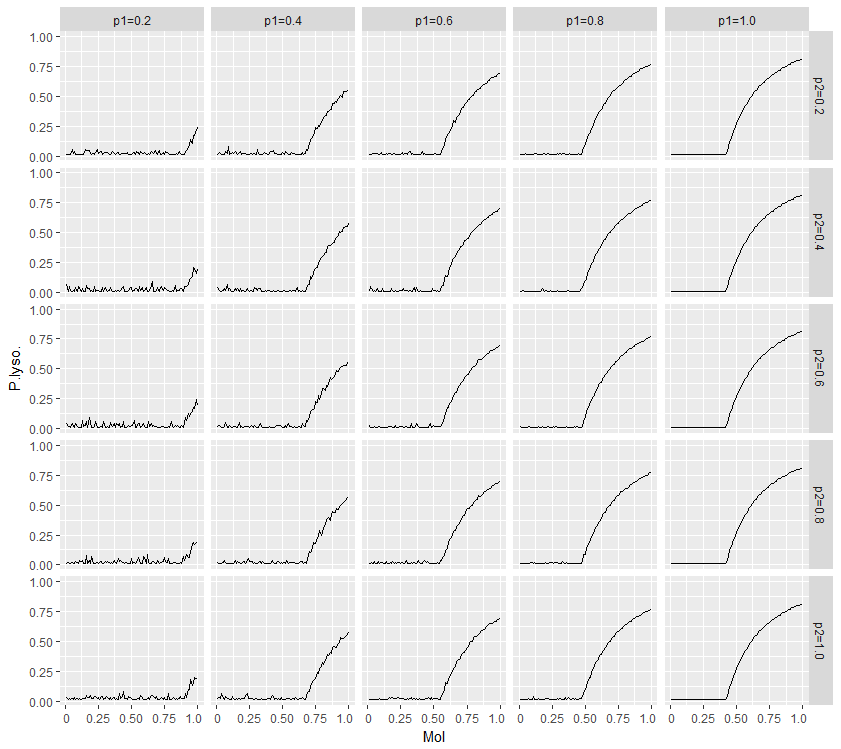
\includegraphics[width=160mm]{facet_grid4.png}
\caption{\color{Gray} \textbf{A Trellis plot displaying the variation in $P_{lyso}$ vs $MoI$ trends as a function of $p_1$ and $p_2$ for a given value of $\lambda_p$ and $\lambda_b$ ($\lambda_p$ = 3, $\lambda_b$ = 0.1)}. The foremost observation here is the variation of the curve as a function of $p_1$. As the environment becomes better for phages, more and more phages opt for lysogeny. The change in the trend as the bacterial environments improve is subtler and is better perceived from the area under the graph.}

\label{fig2} % \label works only AFTER \caption within figure environment

\end{figure}
\newpage
Experimentally, research has shown that the lysis-lysogeny decision varies not only from species to species, but is also dependent on a variety of other factors including but not limited to multiplicity of infection, chemical environment, cell size, and location of inserted phage\cite{kourilsky1973lysogenization}, \cite{kourilsky1975lysogenization}, \cite{zeng2010decision}. The results. The problem that we try to address has been experimentally tested, albeit with the variation of different parameters \cite{kourilsky1973lysogenization}, \cite{zeng2010decision}. Our results match closely the results obtained in \cite{zeng2010decision} (Figure 4A) and are qualitatively similar to the results presented in \cite{kourilsky1973lysogenization} (Figure 2). It is futile to to attempt creating a model that would match the exact data points presented in \cite{kourilsky1973lysogenization} since the data varies greatly for different phage samples and chemical composition of the environment.


\section*{Discussion}

In this paper we have tried to model the impact of environmental factors and the $MoI$ on the optimal lysogenic propensity. We look at the lysis versus lysogeny decision from the point of view of long-term coexistence, a novel approach that hasn't yet been documented elsewhere. By selecting lysogenic propensities that lead to a resultant $MoI$ of 1, we find that the results obtained match qualitatively with experimental data and a more exact matching should be possible by using experimentally noted values for degradation, replication, and amplification rates. 

When the environment is more prone to bad episodes, the phages are more likely to opt for lysogeny. This can be seen as an example of bet-hedging, a concept that has been applied to the study of lysogeny in phages by \cite{avlund2009phage}, \cite{veening2008bistability}, \cite{mittler1996evolution}. Here, we evaluate the effects of various parameters considering bad phage and bacterial environments since restricting the study to good environments limits the observed variation due to change in parameters, as seen in Figure \ref{fig1}. Future work work would involve understanding the effect of the bad bacterial environments on the coexistence in more detail and the linking of our approach to the activation and repression of the lysogenic pathway.


%\clearpage

\section*{Miscellaneous Information}
All the related code is available on \href{https://github.com/DevangThakkar/optimal_phage/tree/master/Run4}{Github}. Queries regarding the same may be directed to devangthakkar [at] iitb [dot] ac [dot] in

%These commands reset the figure counter and add "S" to the figure caption (e.g. "Figure S1"). This is in case you want to add actual figures and not just captions.
\nolinenumbers

%This is where your bibliography is generated. Make sure that your .bib file is actually called library.bib
\bibliography{library}

%This defines the bibliographies style. Search online for a list of available styles.
\bibliographystyle{ieeetr}

\end{document}

